\documentclass[12pt,a4paper]{article}

% --- Page Layout -------------------------------------------------------------
\usepackage[a4paper, margin=0.8in, headheight=14pt]{geometry}

% --- Fonts (XeLaTeX) ---------------------------------------------------------
\usepackage{fontspec}
\usepackage{unicode-math}
\setmainfont{TeX Gyre Pagella}
\setmonofont[Scale=0.88]{TeX Gyre Cursor}
\setmathfont{Latin Modern Math}

% --- Packages ---------------------------------------------------------------
\usepackage{xcolor}
\usepackage{titlesec}
\usepackage{enumitem}
\usepackage{tabularx}
\usepackage{booktabs}
\usepackage{array}
\usepackage{amsmath}
\usepackage{tikz}
\usetikzlibrary{shapes.geometric, arrows.meta, positioning, calc, fit, decorations.pathreplacing}
\usepackage{tcolorbox}
\tcbuselibrary{skins, breakable}
\usepackage{hyperref}
\usepackage{fancyhdr}
\usepackage{graphicx}
\usepackage{microtype}
\hyphenpenalty=10000
\exhyphenpenalty=10000
\sloppy
\usepackage{caption}
\usepackage{setspace}
\usepackage{multirow}
\usepackage{tocloft}

% --- Q&A helper --------------------------------------------------------------
\newcommand{\Q}[1]{\textbf{#1}\par\noindent\ignorespaces}

% --- Colour Palette ----------------------------------------------------------
\definecolor{myred}{RGB}{196,30,58}
\definecolor{mydark}{RGB}{30,30,50}
\definecolor{mygreen}{RGB}{14,120,80}
\definecolor{myteal}{RGB}{0,130,140}
\definecolor{myamber}{RGB}{180,100,0}
\definecolor{mypurple}{RGB}{100,30,160}
\definecolor{mygray}{RGB}{246,247,249}
\definecolor{mgframe}{RGB}{180,185,200}
\definecolor{watermark}{RGB}{145,150,170}
\definecolor{hdrred}{RGB}{250,232,235}
\definecolor{hdrgreen}{RGB}{220,244,233}
\definecolor{hdrteal}{RGB}{220,242,244}
\definecolor{hdramber}{RGB}{253,242,215}
\definecolor{hdrpurple}{RGB}{238,228,255}
\definecolor{hdrgray}{RGB}{238,240,245}
\definecolor{rowalt}{RGB}{250,251,253}

% --- Section Formatting ------------------------------------------------------
\titleformat{\section}
  {\large\bfseries\color{myred}}{\thesection.}{0.5em}{}
  [\vspace{1pt}{\color{myred}\rule{\linewidth}{0.8pt}}]
\titleformat{\subsection}
  {\normalsize\bfseries\color{myteal}}{\thesubsection}{0.5em}{}
\titlespacing*{\section}{0pt}{18pt}{7pt}
\titlespacing*{\subsection}{0pt}{11pt}{4pt}

% --- Paragraph ---------------------------------------------------------------
\setlength{\parindent}{0pt}
\setlength{\parskip}{4pt}

% --- TOC Styling -------------------------------------------------------------
\renewcommand{\cfttoctitlefont}{\large\bfseries\color{myred}}
\renewcommand{\cftaftertoctitle}{\par\noindent{\color{myred}\rule{\linewidth}{0.8pt}}}
\setlength{\cftbeforetoctitleskip}{0pt}
\setlength{\cftaftertoctitleskip}{6pt}
\renewcommand{\cftsecfont}{\normalsize\bfseries\color{mydark}}
\renewcommand{\cftsecpagefont}{\normalsize\bfseries\color{mydark}}
\renewcommand{\cftsecleader}{\cftdotfill{\cftdotsep}}
\setlength{\cftbeforesecskip}{7pt}
\renewcommand{\cftsubsecfont}{\small\color{mydark}}
\renewcommand{\cftsubsecpagefont}{\small\color{mydark}}
\setlength{\cftbeforesubsecskip}{3pt}
\setlength{\cftsubsecindent}{1.4em}

% --- Table helpers -----------------------------------------------------------
\renewcommand{\arraystretch}{1.45}
\setlength{\tabcolsep}{6pt}
\newcolumntype{B}[1]{>{\small\bfseries\raggedright\arraybackslash}m{#1}}
\newcolumntype{Y}{>{\small\raggedright\arraybackslash}X}
\renewcommand{\tabularxcolumn}[1]{m{#1}}

% --- Header / Footer ---------------------------------------------------------
\pagestyle{fancy}
\fancyhf{}
\fancyhead[L]{\small\color{myred}\textbf{BS-CH101}\;\color{mydark}--- Chemistry-I}
\fancyhead[R]{\small\color{myteal}\textbf{Module 6 Notes}}
\fancyfoot[C]{\small\color{mydark}\thepage}
\fancyfoot[R]{\small\color{watermark}\textit{\copyright\ Biraj}}
\renewcommand{\headrulewidth}{0.5pt}
\renewcommand{\footrulewidth}{0.3pt}

% --- Hyperref ---------------------------------------------------------------
\hypersetup{
  colorlinks=true, linkcolor=myteal, urlcolor=myteal,
  pdfauthor={Biraj Sarkar},
  pdftitle={BS-CH101 --- Module 6 Notes}
}

% --- tcolorbox styles --------------------------------------------------------
\tcbset{
  tikzbox/.style={
    colback=mygray, colframe=mgframe, boxrule=0.6pt, arc=4pt,
    left=8pt, right=8pt, top=6pt, bottom=6pt,
    colbacktitle=mgframe, coltitle=mydark,
    fonttitle=\small\bfseries
  },
  defbox/.style={
    colback=hdrgreen, colframe=mygreen, boxrule=0.8pt, arc=4pt,
    left=9pt, right=9pt, top=6pt, bottom=6pt,
    colbacktitle=mygreen, coltitle=white,
    fonttitle=\small\bfseries
  },
  formulabox/.style={
    colback=hdrteal, colframe=myteal, boxrule=0.8pt, arc=4pt,
    left=9pt, right=9pt, top=7pt, bottom=7pt,
    colbacktitle=myteal, coltitle=white,
    fonttitle=\small\bfseries
  },
  examplebox/.style={
    colback=hdramber, colframe=myamber, boxrule=0.8pt, arc=4pt,
    left=9pt, right=9pt, top=6pt, bottom=6pt,
    colbacktitle=myamber, coltitle=white,
    fonttitle=\small\bfseries
  },
  masonbox/.style={
    colback=hdrpurple, colframe=mypurple, boxrule=0.8pt, arc=4pt,
    left=9pt, right=9pt, top=6pt, bottom=6pt,
    colbacktitle=mypurple, coltitle=white,
    fonttitle=\small\bfseries
  },
  exambox/.style={
    colback=hdrpurple, colframe=mypurple, boxrule=1pt, arc=5pt,
    left=10pt, right=10pt, top=8pt, bottom=8pt,
    colbacktitle=mypurple, coltitle=white,
    fonttitle=\bfseries,
    breakable, title after break={\textbf{Frequently Asked / Viva Questions (contd.)}}}
}
\tcbset{breakable}

% --- TikZ styles -------------------------------------------------------------
\tikzset{
  block/.style={rectangle, draw=myteal, fill=hdrteal,
    text width=2.4cm, align=center, minimum height=0.95cm,
    font=\small, rounded corners=3pt, line width=0.7pt},
  redblock/.style={rectangle, draw=myred, fill=hdrred,
    text width=2.4cm, align=center, minimum height=0.95cm,
    font=\small, rounded corners=3pt, line width=0.7pt},
  netnode/.style={rectangle, draw=myteal, fill=hdrteal,
    text width=1.5cm, align=center, minimum height=0.8cm,
    font=\small, rounded corners=3pt, line width=0.7pt},
  sumjunc/.style={circle, draw=myamber, fill=hdramber,
    minimum size=0.62cm, font=\small, line width=0.8pt},
  snode/.style={circle, draw=mypurple, fill=hdrpurple,
    minimum size=0.55cm, font=\footnotesize, line width=0.7pt},
  arrow/.style={-Stealth, thick, color=mydark},
  redarrow/.style={-Stealth, thick, color=myred},
  line/.style={thick, color=mydark}
}

\begin{document}

\begin{center}
  {\LARGE\bfseries\color{myred} BS-CH101 / BS-CH201 --- Chemistry-I}\\[5pt]
  {\normalsize\color{mydark} Semester I \quad$\bullet$\quad 3L:1T:0P \quad$\bullet$\quad 4 Credits}\\[3pt]
  {\normalsize\color{myteal}\textbf{Module 6 Exam Notes: Stereochemistry}}\\[3pt]
  {\small\color{mydark} CGEC \;$|$\; B.Tech ECE (2023--27) \;$|$\; \textit{Biraj Sarkar}}
\end{center}
\vspace{2pt}
\noindent{\color{myred}\rule{\linewidth}{1.5pt}}
\vspace{2pt}

\hypersetup{linkcolor=mydark}
\tableofcontents
\hypersetup{linkcolor=myteal}
\newpage
% ===============================================================================
\section{Stereochemistry}
% ===============================================================================

\begin{tcolorbox}[defbox]
\textbf{Stereochemistry} is the study of three-dimensional arrangement of atoms in molecules and how this arrangement affects physical, chemical, and biological properties.
\end{tcolorbox}

\subsection{Representations of Three-Dimensional Structures}
Three-dimensional structures are represented using wedge-dash, Fischer projection, Newman projection, and sawhorse projection.

\begin{tcolorbox}[tikzbox, title={Wedge-Dash Representation Around a Tetrahedral Carbon}]
\centering
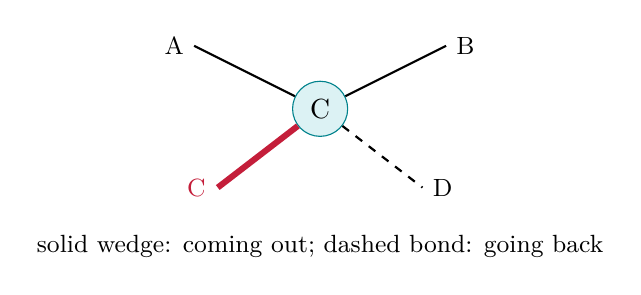
\begin{tikzpicture}[scale=1.0]
  \node[circle, draw=myteal, fill=hdrteal, minimum size=0.7cm] (c) at (0,0) {C};
  \draw[thick] (c) -- (-1.6,0.8) node[left,font=\small] {A};
  \draw[thick] (c) -- (1.6,0.8) node[right,font=\small] {B};
  \draw[line width=2.2pt,myred] (c) -- (-1.3,-1.0) node[left,font=\small] {C};
  \draw[dashed,thick] (c) -- (1.3,-1.0) node[right,font=\small] {D};
  \node[font=\small] at (0,-1.75) {solid wedge: coming out; dashed bond: going back};
\end{tikzpicture}
\end{tcolorbox}

\subsection{Structural Isomers and Stereoisomers}
Structural isomers differ in connectivity, whereas stereoisomers have same connectivity but different spatial arrangement.

\begin{tabularx}{\linewidth}{|B{3cm}|Y|Y|}
\hline
\textbf{Type} & \textbf{Meaning} & \textbf{Example} \\
\hline
Chain isomerism & Different carbon skeleton & n-butane and isobutane \\
\hline
Position isomerism & Functional group at different position & 1-propanol and 2-propanol \\
\hline
Geometrical isomerism & Different arrangement around double bond/ring & cis-2-butene and trans-2-butene \\
\hline
Optical isomerism & Non-superimposable mirror images & lactic acid enantiomers \\
\hline
\end{tabularx}

\subsection{Chirality, Enantiomers and Diastereomers}
A molecule is chiral if it is not superimposable on its mirror image. A common cause is a carbon attached to four different groups.

\begin{tcolorbox}[defbox]
\textbf{Enantiomers} are non-superimposable mirror-image stereoisomers. \textbf{Diastereomers} are stereoisomers that are not mirror images.
\end{tcolorbox}

\subsection{Optical Activity and Absolute Configuration}
Optically active substances rotate plane-polarized light. Absolute configuration is assigned by Cahn-Ingold-Prelog rules.

\begin{tcolorbox}[formulabox, title={Specific Rotation}]
\[
[\alpha]_{\lambda}^{T}=\frac{\alpha}{lc}
\]
where $\alpha$ is observed rotation in degrees, $l$ is path length in dm, and $c$ is concentration in $\mathrm{g\,mL^{-1}}$.
\end{tcolorbox}

\subsection{Conformational Analysis}
Conformations arise by rotation about single bonds. Ethane has staggered and eclipsed conformations; staggered is more stable due to lower torsional strain.

\begin{tcolorbox}[tikzbox, title={Ethane Conformations: Staggered and Eclipsed}]
\centering
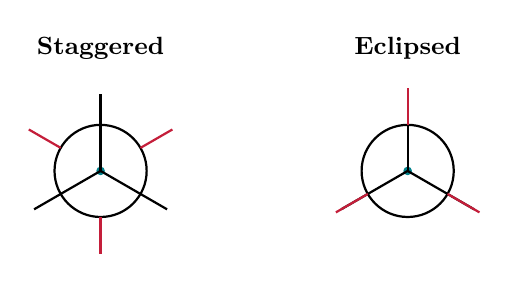
\begin{tikzpicture}[scale=0.78]
  \node[font=\small\bfseries] at (0,2.0) {Staggered};
  \draw[thick] (0,0) circle (0.75);
  \fill[myteal] (0,0) circle (2pt);
  \foreach \a in {90,210,330} \draw[thick] (0,0) -- (\a:1.25);
  \foreach \a in {30,150,270} \draw[thick,myred] (\a:0.75) -- (\a:1.35);
  \node[font=\small\bfseries] at (5,2.0) {Eclipsed};
  \draw[thick] (5,0) circle (0.75);
  \fill[myteal] (5,0) circle (2pt);
  \foreach \a in {90,210,330} {
    \draw[thick] (5,0) -- ($(5,0)+(\a:1.25)$);
    \draw[thick,myred] ($(5,0)+(\a:0.75)$) -- ($(5,0)+(\a:1.35)$);
  }
\end{tikzpicture}
\end{tcolorbox}

\subsection{Isomerism in Transition Metal Compounds}
Coordination compounds show geometrical, optical, linkage, ionization, and coordination isomerism. Square planar and octahedral complexes commonly show cis-trans isomerism.

\begin{tcolorbox}[exambox, title={Exam Points}]
\begin{itemize}[leftmargin=*, itemsep=2pt, topsep=2pt]
  \item Always distinguish structural isomerism from stereoisomerism.
  \item In optical isomerism, mention chirality and non-superimposable mirror images.
  \item CIP assignment needs priority order before clockwise/anticlockwise decision.
  \item For conformational analysis, compare stability using torsional strain.
\end{itemize}
\end{tcolorbox}

% ===============================================================================
\section{Detailed Stereochemical Analysis}
% ===============================================================================

\subsection{Fischer Projection Rules}
Fischer projections are used mainly for molecules with chiral carbon chains. Horizontal bonds come out of the plane toward the viewer; vertical bonds go behind the plane.

\begin{tcolorbox}[tikzbox, title={Fischer Projection Convention}]
\centering
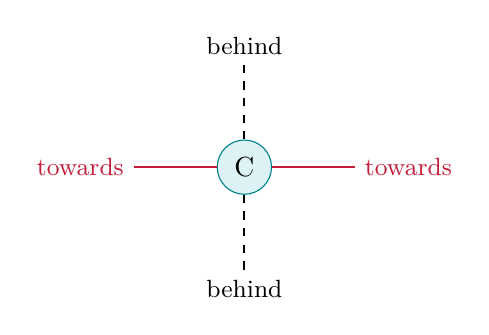
\begin{tikzpicture}[scale=1.0]
  \node[circle, draw=myteal, fill=hdrteal, minimum size=0.6cm] (c) at (0,0) {C};
  \draw[thick,myred] (c) -- (-1.4,0) node[left,font=\small] {towards};
  \draw[thick,myred] (c) -- (1.4,0) node[right,font=\small] {towards};
  \draw[thick,dashed] (c) -- (0,1.3) node[above,font=\small] {behind};
  \draw[thick,dashed] (c) -- (0,-1.3) node[below,font=\small] {behind};
\end{tikzpicture}
\end{tcolorbox}

\begin{tcolorbox}[masonbox, title={Rules for Fischer Projections}]
\begin{itemize}[leftmargin=*, itemsep=2pt, topsep=2pt]
  \item Rotation by $180^\circ$ gives the same molecule.
  \item Rotation by $90^\circ$ gives a different configuration and is not allowed.
  \item Interchanging any two groups once inverts configuration.
  \item Interchanging two pairs of groups gives the original configuration.
\end{itemize}
\end{tcolorbox}

\subsection{Assigning R and S Configuration}
Cahn-Ingold-Prelog priority rules:
\begin{enumerate}[leftmargin=*, itemsep=3pt, topsep=2pt]
  \item Atom directly attached with higher atomic number gets higher priority.
  \item If first atoms are same, compare the next set of attached atoms.
  \item Multiple bonds are treated as equivalent single bonds to duplicate atoms.
  \item View the molecule with the lowest priority group pointing away.
  \item Clockwise order $1\rightarrow2\rightarrow3$ is $R$; anticlockwise is $S$.
\end{enumerate}

\begin{tcolorbox}[examplebox, title={Worked Method: R/S Assignment}]
For a chiral carbon attached to $\mathrm{Br}$, $\mathrm{Cl}$, $\mathrm{CH_3}$, and $\mathrm{H}$:
\[
\mathrm{Br}>\mathrm{Cl}>\mathrm{C}>\mathrm{H}
\]
Place $\mathrm{H}$ away from the viewer. If the order Br $\rightarrow$ Cl $\rightarrow$ $\mathrm{CH_3}$ is clockwise, the configuration is $R$; if anticlockwise, it is $S$.
\end{tcolorbox}

\subsection{Geometrical Isomerism: E/Z and Cis/Trans}
Geometrical isomerism occurs due to restricted rotation around a double bond or within rings. Cis/trans notation is used for simple cases; E/Z notation is used when each double-bond carbon has two different groups.

\begin{tabularx}{\linewidth}{|B{3.2cm}|Y|Y|}
\hline
\textbf{Notation} & \textbf{Meaning} & \textbf{Use case} \\
\hline
Cis & Similar groups on same side & Simple alkenes or rings \\
\hline
Trans & Similar groups on opposite sides & Simple alkenes or rings \\
\hline
E & Higher-priority groups on opposite sides & General alkenes by CIP rule \\
\hline
Z & Higher-priority groups on same side & General alkenes by CIP rule \\
\hline
\end{tabularx}

\subsection{Meso Compounds}
A meso compound contains chiral centres but is optically inactive due to internal symmetry. It is superimposable on its mirror image because optical rotations of two halves cancel internally.

\begin{tcolorbox}[defbox]
\textbf{Meso compound:} An achiral molecule with two or more stereocentres and an internal plane of symmetry.
\end{tcolorbox}

\subsection{Conformational Analysis of Butane}
Butane has anti, gauche, and eclipsed conformations. Anti is most stable because bulky methyl groups are far apart.

\begin{tabularx}{\linewidth}{|B{3cm}|Y|Y|}
\hline
\textbf{Conformation} & \textbf{Dihedral angle between methyl groups} & \textbf{Relative stability} \\
\hline
Anti staggered & $180^\circ$ & Most stable \\
\hline
Gauche staggered & $60^\circ$ & Less stable due to steric repulsion \\
\hline
Eclipsed & $0^\circ$ or $120^\circ$ & Least stable due to torsional strain \\
\hline
\end{tabularx}

\begin{tcolorbox}[examplebox, title={Specific Rotation Numerical}]
If observed rotation $\alpha=+6^\circ$, path length $l=2\ \mathrm{dm}$, and concentration $c=0.5\ \mathrm{g\,mL^{-1}}$:
\[
[\alpha]=\frac{\alpha}{lc}=\frac{6}{2\times0.5}=+6^\circ
\]
\end{tcolorbox}

\subsection{Coordination Compound Stereoisomerism}
Square planar complexes of type $\mathrm{MA_2B_2}$ show cis-trans isomerism. Octahedral complexes may show cis-trans, fac-mer, and optical isomerism depending on ligand arrangement.

\begin{tabularx}{\linewidth}{|B{3cm}|Y|Y|}
\hline
\textbf{Complex type} & \textbf{Possible isomerism} & \textbf{Example pattern} \\
\hline
Square planar $\mathrm{MA_2B_2}$ & Cis-trans & $\mathrm{[Pt(NH_3)_2Cl_2]}$ \\
\hline
Octahedral $\mathrm{MA_4B_2}$ & Cis-trans & Two B ligands adjacent or opposite \\
\hline
Octahedral $\mathrm{MA_3B_3}$ & fac-mer & Three same ligands on one face or meridian \\
\hline
\end{tabularx}

\begin{tcolorbox}[masonbox, title={Stereochemistry Answer Checklist}]
\begin{enumerate}[leftmargin=*, itemsep=3pt, topsep=2pt]
  \item Identify whether connectivity changes or only spatial arrangement changes.
  \item Check for chirality, plane of symmetry, and mirror-image relation.
  \item Use CIP rules for R/S or E/Z configuration.
  \item Mention optical activity only after checking symmetry.
\end{enumerate}
\end{tcolorbox}

\subsection{Number of Stereoisomers}
For a molecule with $n$ independent chiral centres, the maximum number of stereoisomers is:
\[
2^n
\]
If the molecule has internal symmetry, the actual number is less due to meso forms.

\begin{tcolorbox}[examplebox, title={Solved Example: Number of Stereoisomers}]
A molecule has two chiral centres and no plane of symmetry.
\[
\text{Maximum stereoisomers}=2^2=4
\]
These are arranged as two pairs of enantiomers. If a plane of symmetry exists, one or more meso forms reduce the total count.
\end{tcolorbox}

\subsection{Resolution of Racemic Mixtures}
A racemic mixture contains equal amounts of two enantiomers and is optically inactive. Resolution means separation of enantiomers.

\begin{tabularx}{\linewidth}{|B{3.2cm}|Y|Y|}
\hline
\textbf{Method} & \textbf{Principle} & \textbf{Use} \\
\hline
Mechanical separation & Physical separation of crystals & Rare; possible if crystals differ visibly \\
\hline
Chemical resolution & Formation of diastereomeric salts & Common laboratory method \\
\hline
Biochemical resolution & Enzyme reacts with one enantiomer faster & High selectivity \\
\hline
Chromatographic resolution & Chiral stationary phase separates enantiomers & Analytical and preparative use \\
\hline
\end{tabularx}

\subsection{Optical Purity and Enantiomeric Excess}
Optical purity compares observed rotation with rotation of the pure enantiomer.

\begin{tcolorbox}[formulabox, title={Optical Purity}]
\[
\text{Optical purity}=\frac{\alpha_{\mathrm{observed}}}{\alpha_{\mathrm{pure}}}\times100\%
\]
For a two-enantiomer mixture, optical purity is equal to enantiomeric excess.
\end{tcolorbox}

\begin{tcolorbox}[examplebox, title={Solved Example: Enantiomeric Excess}]
If pure enantiomer has specific rotation $+40^\circ$ and mixture shows $+20^\circ$:
\[
\text{optical purity}=\frac{20}{40}\times100=50\%
\]
So enantiomeric excess is $50\%$. The mixture contains $75\%$ major enantiomer and $25\%$ minor enantiomer.
\end{tcolorbox}

\subsection{Sequence Rules for Double Bonds: E/Z Worked Method}
For each double-bond carbon, assign priority to its two substituents using CIP rules. If the two higher-priority groups are on the same side, the alkene is $Z$; if opposite, it is $E$.

\begin{tcolorbox}[examplebox, title={Worked Method: E/Z Assignment}]
For $\mathrm{CH_3CH=CHCl}$, compare substituents on each double-bond carbon. On the left carbon, $\mathrm{CH_3}$ has higher priority than H. On the right carbon, Cl has higher priority than H. If $\mathrm{CH_3}$ and Cl are on opposite sides, the configuration is $E$; if same side, it is $Z$.
\end{tcolorbox}

\subsection{Energy Profile of Butane Rotation}
Rotation about the central C--C bond of butane gives different conformations. Anti is most stable; fully eclipsed is least stable.

\begin{tcolorbox}[tikzbox, title={Qualitative Energy Profile for Butane Rotation}]
\centering
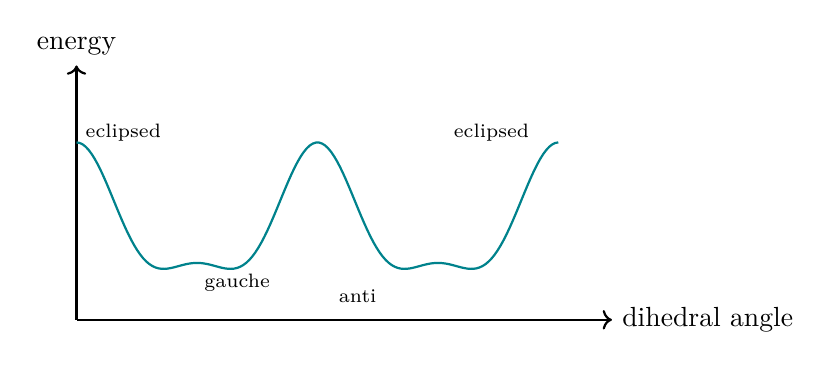
\begin{tikzpicture}[scale=0.85]
  \draw[->, thick] (0,0) -- (8,0) node[right] {dihedral angle};
  \draw[->, thick] (0,0) -- (0,3.8) node[above] {energy};
  \draw[myteal, thick, domain=0:7.2, samples=160]
    plot(\x,{1.4+0.9*cos(100*\x)+0.35*cos(200*\x)});
  \node[font=\scriptsize] at (0.7,2.8) {eclipsed};
  \node[font=\scriptsize] at (2.4,0.55) {gauche};
  \node[font=\scriptsize] at (4.2,0.35) {anti};
  \node[font=\scriptsize] at (6.2,2.8) {eclipsed};
\end{tikzpicture}
\end{tcolorbox}

\subsection{Stereochemistry in Biological and Drug Action}
Many drug molecules are chiral, and different enantiomers can show different biological activity because enzymes and receptors are chiral environments.

\begin{tabularx}{\linewidth}{|B{3cm}|Y|}
\hline
\textbf{Point} & \textbf{Importance} \\
\hline
Different receptor fit & One enantiomer may bind better than the other \\
\hline
Different metabolism & Enzymes may break down enantiomers at different rates \\
\hline
Different toxicity & One enantiomer may be useful while the other causes side effects \\
\hline
Quality control & Optical purity matters in pharmaceutical synthesis \\
\hline
\end{tabularx}

\begin{tcolorbox}[masonbox, title={Previous-Year Style Questions}]
\begin{enumerate}[leftmargin=*, itemsep=4pt, topsep=2pt]
  \item Explain chirality, enantiomers and diastereomers with examples.
  \item State CIP rules and assign R/S configuration for a given molecule.
  \item Explain optical activity, specific rotation and racemic mixture.
  \item Compare conformations of ethane and butane.
  \item Discuss geometrical and optical isomerism in coordination compounds.
\end{enumerate}
\end{tcolorbox}
\newpage
\begin{center}
  {\large\bfseries\color{myred} Quick Revision --- Module 6}\\[3pt]
  {\small\color{mydark} Stereochemistry $|$ BS-CH101}
\end{center}
\noindent{\color{myred}\rule{\linewidth}{1.2pt}}
\vspace{4pt}

\begin{tcolorbox}[formulabox, title={Key Formulas at a Glance}]
\begin{tabularx}{\linewidth}{|B{4.0cm}|Y|}
\hline
\textbf{Formula / Rule} & \textbf{Meaning} \\
\hline
$[\alpha]_{\lambda}^{T}=\displaystyle\frac{\alpha}{lc}$ & Specific rotation of optically active compound. \\
\hline
$\text{enantiomeric excess}=\displaystyle\frac{|R-S|}{R+S}\times100\%$ & Optical purity of a mixture. \\
\hline
$\Delta E=E_{\mathrm{eclipsed}}-E_{\mathrm{staggered}}$ & Torsional energy barrier in conformational analysis. \\
\hline
CIP priority & Higher atomic number gets higher priority. \\
\hline
\end{tabularx}
\end{tcolorbox}

\begin{tcolorbox}[defbox, title={One-Line Definitions}]
\begin{itemize}[leftmargin=*, itemsep=2pt, topsep=2pt]
  \item \textbf{Stereoisomers:} Same connectivity but different spatial arrangement.
  \item \textbf{Chiral molecule:} Molecule not superimposable on its mirror image.
  \item \textbf{Enantiomers:} Non-superimposable mirror-image isomers.
  \item \textbf{Diastereomers:} Stereoisomers that are not mirror images.
  \item \textbf{Optical activity:} Ability to rotate plane-polarized light.
  \item \textbf{Conformation:} Spatial arrangement formed by rotation about single bond.
  \item \textbf{Racemic mixture:} Equimolar mixture of two enantiomers.
\end{itemize}
\end{tcolorbox}

\begin{tcolorbox}[exambox, title={Frequently Asked / Viva Questions}]
\begin{enumerate}[topsep=0pt, label=\textbf{Q\arabic*.}, itemsep=5pt]
  \item \Q{What is stereochemistry?}
    Study of three-dimensional arrangement of atoms in molecules.
  \item \Q{What is chirality?}
    Non-superimposability of a molecule on its mirror image.
  \item \Q{Define enantiomers.}
    Enantiomers are non-superimposable mirror-image stereoisomers.
  \item \Q{Define diastereomers.}
    Diastereomers are stereoisomers that are not mirror images.
  \item \Q{What is optical activity?}
    Rotation of plane-polarized light by a chiral substance.
  \item \Q{What is a racemic mixture?}
    A 1:1 mixture of enantiomers having zero net optical rotation.
  \item \Q{What does R/S configuration indicate?}
    It gives absolute three-dimensional arrangement around a chiral centre.
  \item \Q{Why is staggered ethane more stable than eclipsed ethane?}
    Staggered conformation has minimum torsional repulsion.
  \item \Q{Name isomerism in coordination compounds.}
    Geometrical, optical, linkage, ionization, and coordination isomerism.
  \item \Q{What is geometrical isomerism?}
    Isomerism due to restricted rotation causing cis-trans or fac-mer forms.
\end{enumerate}
\end{tcolorbox}

\begin{tcolorbox}[tikzbox, title={Summary Reference Table}]
\begin{tabularx}{\linewidth}{|B{3cm}|Y|Y|}
\hline
\textbf{Pair} & \textbf{Relation} & \textbf{Key difference} \\
\hline
Structural isomers & Different connectivity & Different bonding sequence \\
\hline
Enantiomers & Mirror images & Equal and opposite optical rotation \\
\hline
Diastereomers & Not mirror images & Different physical properties \\
\hline
Conformers & Rotation about single bond & Interconvert without bond breaking \\
\hline
\end{tabularx}
\end{tcolorbox}

\end{document}
